\Transcb{yellow}{blue}{Gravity as a geometrical effect}
\onecolumn
\begin{itemize}
\item Deflection of light in a gravitational field
\item[] Not corresponding to Newtonian gravity formula
\item[] Ultimate proof that all particles experience the same $\vec{a}$ irrespective of $m$
\item Einstein's idea concerning gravitational path deflection
\item[] Consider a particle traveling in a straight line over a flat rubber sheet
\item[] Put a heavy object on the rubber sheet $\rightarrow$ sheet stretches and curves
\item[] $\rightarrow$ The particle will now follow a curved path on the sheet
\item[] {\blue Gravitational path deflection is due to curvature of space}
\item Similar reasoning for the time coordinates
\item[] {\blue Gravitational time dilation is due to curvature of time}
\end{itemize}
%
\begin{center}
\colorbox{yellow}{Relativistic viewpoint on gravity}\\[3mm]
{\red \shabox{Gravity is a geometric effect due to curvature of space-time}}\\[3mm]
{\red \shabox{The presence of mass introduces a curvature in space-time}}
\end{center}

\Tr
\twocolumn[\begin{center}
            {\blue How to introduce curvature in space-time in accordance with observations ?}
            \vspace*{3mm}
           \end{center}]
\begin{itemize}
\item Detailed look at the equivalence principle
\item[] Frame $S$ in free fall with two objects at rest
\item[$\ast$] {\red Can the earth gravity stay "hidden" ?}
\item[] $|\vec{g}|$ must be constant in $S \rightarrow \d y$ small
\item[] $g_{x}$ must be small $\rightarrow \d x$ small
\item[] Observation time $T$ must be small
\item[] \begin{center}\colorbox{yellow}{The Equivalence Principle}\end{center}
{\red
\item[] Experiments performed in a sufficiently\\
        small freely falling laboratory, over a\\
        sufficiently short time, yield results that are\\
        indistinguishable from those of the same\\
        experiments performed in an inertial frame in empty space.
}
\end{itemize}

\newpage

\begin{center}
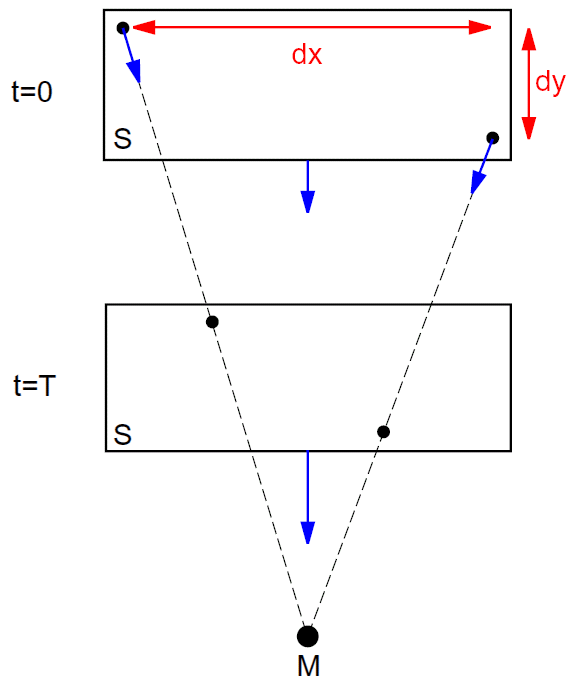
\includegraphics[keepaspectratio,height=14cm]{equivalence2}
\end{center}

\Tr
\twocolumn[\begin{center}
            {\blue Linking the Equivalence Principle with relativity}
            \vspace*{5mm}
           \end{center}]
%
\begin{itemize}
\item Relativistic description of an {\red inertial frame}
\item[] It's all included in the metric
\item[] $\d s^{2}=(c\d t)^{2}-\d\vec{r}^{\,2}$
\item[] As 4-vectors~: {\red $\d s^{2}=\eta_{\mu\nu}\,\d x^{\mu}\,\d x^{\nu}$}
\item[] with $\eta_{\mu\nu}=\text{diag}(1,-1,-1,-1)$
\item In the presence of gravity~:
\item[] Freely falling frame is only locally inertial
\item[] $\rightarrow$ All other locations in space-time have~:
\item[] {\blue $\qquad \d s^{2}=g_{\mu\nu}(\Fvec{x})\,\d x^{\mu}\,\d x^{\nu}$}
\item[] $\Fvec{x} \equiv$ location in space-time
\end{itemize}

\newpage

\begin{itemize}
\item[] \begin{center}\colorbox{yellow}{Description of space-time curvature}\end{center}
{\red
\item[] Introduce metric tensor $g_{\mu\nu}(\Fvec{x})$ of which the components
        depend on the location in space-time 
}
\item Equivalence Principle~: $S \rightarrow S^{\,\prime}$
\item[] $g_{\mu\nu}(\Fvec{x}) \rightarrow g_{\mu\nu}^{\,\prime}(\Fvec{x}^{\,\prime})=\eta_{\mu\nu}$
\item Consequences~:
{\blue
\item[] $g_{\mu\nu}(\Fvec{x})$ must be a symmetric 4x4 matrix
\item[] Always 1 time and 3 space coordinates
}
\item[$\ast$] This is the basis of {\red General Relativity}
\item[] \colorbox{yellow}{What are the components of $g_{\mu\nu}(\Fvec{x})$ ?}
\item[] $\rightarrow$ Need to investigate curvature
\end{itemize}